\documentclass[12pt]{report}

%%% Preamble %%%%%%%%%%%%%%%%%%%%%%%%%%%%%%%%%%%%%%%%%%%%%%%%%%%%%%%%%%%%%%%%%%
\usepackage[T1]{fontenc}
\usepackage[utf8]{inputenc}
\usepackage{times}
\usepackage{geometry}
\geometry{left=1.2in, right=0.9in, top=0.5in, bottom=1.5in}

\usepackage{tikz}
\usepackage{pgfplots}
\pgfplotsset{compat=1.18}
\usepackage{pgf-pie}
\usetikzlibrary{positioning}
\usetikzlibrary{shapes.geometric}
\usetikzlibrary{arrows.meta}

%%% Packages %%%%%%%%%%%%%%%%%%%%%%%%%%%%%%%%%%%%%%%%%%%%%%%%%%%%%%%%%%%%%%%%%%
\usepackage{enumerate}
\usepackage{amsmath}
\usepackage{amsfonts}
\usepackage{amssymb}
\usepackage{amsthm}
\usepackage{float}
\usepackage{url}
\usepackage[numbers]{natbib}  % Using natbib for better citation handling
\usepackage{textcomp}
\usepackage{setspace}
\usepackage{graphicx}
\usepackage[dvipsnames]{xcolor}
\usepackage{hyperref}
\usepackage{makeidx}
\usepackage{listings}
\usepackage{multicol}
\usepackage{courier}
\usepackage{booktabs}
\usepackage{multirow}
\usepackage{adjustbox}
\usepackage{bookmark}
\usepackage{subcaption}
\usepackage{array}

% Hyperref setup
\hypersetup{
    colorlinks=true,
    linkcolor=blue,
    filecolor=magenta,
    urlcolor=cyan,
    pdftitle={Smart Agricultural Advisory Application for Kyera Agricultural Farm, Mbarara District},
    pdfauthor={ATUYAMBE ADAM},
    pdfsubject={Bachelor's Degree Research Proposal in Information Technology},
    pdfkeywords={Smart agriculture, mobile advisory system, weather-pest integration, preventive farming, Uganda},
    bookmarksopen=true,
    bookmarksnumbered=true,
    pdfstartview=FitH
}

% Listings setup
\definecolor{darkgray}{rgb}{0.95,0.95,0.95}
\lstset{
    language=XML,
    basicstyle=\ttfamily\footnotesize,
    keywordstyle=\color{red}\bfseries,
    commentstyle=\color{green!50!black},
    stringstyle=\color{blue},
    showstringspaces=false,
    breaklines=true,
    frame=single,
    backgroundcolor=\color{darkgray}
}

% Float settings
\renewcommand{\topfraction}{0.9}
\renewcommand{\bottomfraction}{0.9}
\renewcommand{\textfraction}{0.1}
\setcounter{topnumber}{10}
\setcounter{bottomnumber}{10}
\setcounter{totalnumber}{10}

% Document formatting
\pagestyle{plain}
\setcounter{tocdepth}{3}
\setcounter{secnumdepth}{3}
\setstretch{1.5} % Good for academic reports

% Theorem environments
\newtheorem{example}{Example}
% amsthm already provides a proof environment

\makeindex

%%% Document Body %%%%%%%%%%%%%%%%%%%%%%%%%%%%%%%%%%%%%%%%%%%%%%%%%%%%%%%%%%%%%

\begin{document}

%%% Title Page %%%%%%%%%%%%%%%%%%%%%%%%%%%%%%%%%%%%%%%%%%%%%%%%%%%%%%%%%%%%%%%%
\begin{titlepage}
    \centering
    \vspace*{1cm}

    {\Huge\bfseries SMART AGRICULTURAL ADVISORY APPLICATION\\}
    \vspace{0.5cm}
    {\Large For Kyera Agricultural Farm, Mbarara District\\}

    \vspace{2cm}

    {\Large A Research Proposal\\}
    \vspace{0.5cm}
    {\Large Submitted in Partial Fulfillment of the Requirements for the\\}
    {\Large Award of Bachelor of Science in Information Technology\\}

    \vspace{2cm}

    {\Large By\\}
    {\Large ADAM ATUYAMBE\\}
    {\large BSc Information Technology Candidate\\}

    \vspace{2cm}

    {\Large University of Saint Joseph Mbarara\\}
    {\Large Faculty of Education and Sciences\\}

    \vspace{2cm}

    {\Large Date: 26TH NOVEMBER 2025\\}

    \vfill
\end{titlepage}

%%% Approval Page %%%%%%%%%%%%%%%%%%%%%%%%%%%%%%%%%%%%%%%%%%%%%%%%%%%%%%%%%%%%%
\newpage
\thispagestyle{empty}
\vspace*{2cm}

\begin{center}
    {\Large\bfseries APPROVAL\\}
\end{center}

\vspace{1cm}

This research work culminating in this research proposal is conducted under my guidance and supervision.

\vspace{2cm}

\begin{center}
\begin{tabular}{p{0.5\textwidth}}
    \hline
    \centering Supervisor's Signature \\
\end{tabular}

\vspace{0.5cm}

\begin{tabular}{p{0.5\textwidth}}
    \centering Mr. Daniel Zziwa \\
    \centering Supervisor \\
\end{tabular}

\vspace{0.5cm}

\begin{tabular}{p{0.5\textwidth}}
    \centering Date: \_\_\_\_\_\_\_\_\_\_\_\_\_\_\_ \\
\end{tabular}
\end{center}

\vfill

%%% Acknowledgements %%%%%%%%%%%%%%%%%%%%%%%%%%%%%%%%%%%%%%%%%%%%%%%%%%%%%%%%%%
\newpage
\thispagestyle{empty}
\chapter*{Acknowledgements}

First and foremost, I give all the glory and honor to the Almighty God for the gift of life, wisdom, and perseverance throughout my academic journey and during the development of this project titled "Smart Agricultural Advisory Application for Kyera Agricultural Farm, Mbarara District." His divine guidance has been my greatest source of strength and inspiration.

I extend my sincere appreciation to my supervisor, Mr. Daniel Zziwa, for his invaluable guidance, continuous support, and encouragement throughout the research and system development process. His constructive feedback, mentorship, and expertise greatly contributed to the successful completion of this work.

My deepest gratitude goes to the management and staff of Kyera Agricultural Farm for their cooperation and for providing the necessary data, insights, and field support that informed the design of this system. Your practical experiences and suggestions shaped the project into a real-world solution for farmers' information needs.

I also wish to acknowledge University of Saint Joseph Mbarara, Faculty of Education and Sciences, for equipping me with the knowledge and technical skills that made this project possible. Special thanks go to my lecturers and classmates for their encouragement and teamwork spirit.

I am forever thankful to my beloved parents Mr. Byaruhanga Adrian and Mrs. Kyomukama Jane, then my brothers for their endless love, prayers, and sacrifices that have brought me to this point.

%%% Dedication %%%%%%%%%%%%%%%%%%%%%%%%%%%%%%%%%%%%%%%%%%%%%%%%%%%%%%%%%%%%%%%%
\newpage
\thispagestyle{empty}
\chapter*{Dedication}

To my beloved parents, Mr. Byaruhanga Adrian and Mrs. Kyomukama Jane, my Research Supervisor Mr. Daniel Zziwa and to my beloved brothers Nasasira Gideon, Nuwahere Gabriel, Nuwampaire Solomon and Nabimanya Innocent.

Thank you for all your support right from when I begun my first year at Campus to offer a Bachelors degree of Science in Information Technology in 2023 to date. You are such a wonderful family to me. Your patience and guidance plus support has made me what I have become today. May the good Lord continue to bless us together for the rest of our lives.

%%% Abstract %%%%%%%%%%%%%%%%%%%%%%%%%%%%%%%%%%%%%%%%%%%%%%%%%%%%%%%%%%%%%%%%%%
\newpage
\pagenumbering{roman}
\setcounter{page}{4}
\chapter*{Abstract}
\addcontentsline{toc}{chapter}{Abstract}

Agriculture remains a fundamental pillar of Uganda's economy, yet smallholder farmers continue to face persistent challenges due to limited access to timely and accurate agricultural information. Traditional extension services, though essential, are often constrained by inadequate staffing, inconsistent coverage, and delays in information dissemination. These gaps undermine farmers' decision-making processes, resulting in reduced productivity, increased vulnerability to pests and diseases, poor market engagement, and overall low farm profitability.

With the rapid growth of mobile and digital technologies in Uganda, there exists a significant opportunity to transform agricultural advisory services through accessible digital platforms. This study proposes the design and implementation of a Smart Agricultural Advisory Application that specifically integrates localized weather forecasts with predictive pest and disease management advisories for farmers at Kyera Agricultural Farm in Mbarara District. Unlike existing fragmented systems, this application bridges the critical disconnect between meteorological data and agricultural risks by providing preventive, weather-triggered alerts.

A mixed-methods approach incorporating interviews, questionnaires, observations, and document review is employed to assess farmers' information needs and establish weather-pest correlations specific to the farm's microclimate. These findings guide the development of a mobile-based system using an agile methodology, ensuring iterative refinement and user-centered validation through prototyping.

The expected outcome is a functional, user-friendly advisory application that enhances farmers' preventive decision-making, improves crop protection outcomes, and promotes agricultural resilience. By addressing the information fragmentation through focused weather-pest integration, this digital platform contributes to modernizing agricultural extension services and advancing sustainable agricultural development in Uganda.

\bigskip
\textbf{Keywords:} Smart agriculture, mobile advisory system, weather-pest integration, preventive farming, digital extension services, Uganda

%%% Table of Contents %%%%%%%%%%%%%%%%%%%%%%%%%%%%%%%%%%%%%%%%%%%%%%%%%%%%%%%%%
\newpage
\tableofcontents

%%% List of Figures %%%%%%%%%%%%%%%%%%%%%%%%%%%%%%%%%%%%%%%%%%%%%%%%%%%%%%%%%%%
\newpage
\listoffigures
\addcontentsline{toc}{chapter}{List of Figures}

%%% List of Tables %%%%%%%%%%%%%%%%%%%%%%%%%%%%%%%%%%%%%%%%%%%%%%%%%%%%%%%%%%%%
\newpage
\listoftables
\addcontentsline{toc}{chapter}{List of Tables}

%%% Main Content %%%%%%%%%%%%%%%%%%%%%%%%%%%%%%%%%%%%%%%%%%%%%%%%%%%%%%%%%%%%%%
\newpage
\pagenumbering{arabic}

\chapter{Introduction}
\label{chapter:introduction}

\section{Introduction and Background of the Study}
Agriculture remains the backbone of Uganda's economy, providing livelihoods for the majority of the population and contributing a substantial share of national output \cite{UBOS2023}. In fiscal year 2022/23, the agricultural sector (agriculture, forestry, and fishing) contributed approximately 23.8 to 24.0\% of Uganda's GDP and employed roughly 68\% of the workforce, highlighting its continued centrality to household incomes and food security \cite{UBOS2023}.

Despite this economic importance, recent trends show that agricultural production growth has not kept pace with demographic pressure and economic expectations. During the last five years, the population increased by 3.3\% per year, while measured agricultural output grew by roughly 2.0\% per year, indicating that agricultural supply expansion is lagging behind population growth and raising concerns about productivity and food security \cite{AgriculturalGrowth2022}. National production indices also show modest improvement (for example, an index of production increase of about 3\% in 2022) \cite{FAO2022}, but these gains are insufficient to close existing yield and income gaps for smallholder farmers \cite{AgriculturalGrowth2022}.

At the same time, Uganda has experienced rapid development in digital and mobile technologies that creates a practical channel for improving agricultural advisory services \cite{ITU2023}. Mobile cellular subscriptions per 100 people rose from approximately 54.0 per 100 in 2015 to about 76.3 per 100 in 2023 an increase of roughly 41.4\% \cite{ITU2023}. Similarly, the share of individuals using the Internet grew from about 5.8\% in 2015 to 15.3\% in 2023 a relative increase of approximately 163.3\% \cite{ITU2023}. These technology adoption trends mean that digital delivery of agricultural information is increasingly feasible for a substantial and growing share of farmers.

The combination of agriculture's continuing economic importance and lagging production growth, alongside rapidly rising mobile and Internet penetration, motivates the development of a mobile, data-driven advisory system for farmers \cite{MAAIF2020}. However, current digital advisory systems provide fragmented information, treating critical factors like weather forecasts and pest/disease management as separate concerns. This fragmentation misses the critical connection between weather patterns and pest/disease outbreaks—a gap that causes preventable crop losses. A Smart Agricultural Advisory Application that integrates localized weather forecasts with predictive pest and disease management advisories can address this gap by delivering preventive, weather-triggered alerts directly to farmers' phones, transforming weather data into actionable agricultural intelligence \cite{MAAIF2020}.

This research therefore seeks to design and implement a Smart Agricultural Advisory Application with a focused thematic scope, using Kyera Agricultural Farm (Mbarara District) as the case study. Kyera is a training and demonstration center with a diverse set of crops and trainees and provides a suitable environment to pilot, evaluate, and refine a mobile advisory system focused on weather-pest integration.

Traditional extension systems, though important, are constrained by limited staffing and resources. The recommended extension worker-to-farmer ratio of 1:500 is far below Uganda's average of 1:1800 \cite{WorldBank2021}. Mobile and digital technologies present opportunities to complement conventional extension. However, current platforms using SMS, apps and call centers typically provide either weather information OR pest/disease advice, missing the critical integration between these factors \cite{FAO2022, ITU2023}. Kyera Agricultural Farm in Mbarara District serves as a relevant case study. As both a demonstration farm and training center, it engages with diverse crops and farmer groups, making it ideal for piloting a Smart Agricultural Advisory Application focused specifically on integrating weather forecasts with pest/disease management.

\section{Problem Statement}
Agriculture has been the cornerstone of Uganda's economy, supporting smallholder farmers who depend on timely and accurate agricultural information to make productive decisions. Historically, farmers relied on traditional advisory channels such as community meetings, radio announcements, and occasional visits from agricultural extension workers. While these methods provided essential guidance, they were often limited in frequency, coverage, precision, and consistency \cite{UBOS2023}. As a result, many farmers frequently received information late or in fragmented form, particularly missing the critical connections between weather forecasts and pest/disease risks.

In recent years, the widespread adoption of mobile phones and digital technologies has created new opportunities for transforming agricultural advisory services. However, despite this technological growth, advisory systems in Uganda remain poorly integrated in their thematic approach. Many smallholder farmers receive weather forecasts through one channel and pest/disease advice through another, with no system connecting these critical factors to provide preventive recommendations \cite{WorldBank2022}. Extension services continue to face significant challenges, including insufficient staffing, limited logistical support, and inadequate geographic coverage \cite{MAAIF2019}. Consequently, farmers continue to make decisions based on disconnected information streams, leading to reactive rather than preventive pest/disease management, resulting in persistent crop losses, and income instability.

Ideally, smallholder farmers should have integrated, actionable agricultural information that connects weather conditions with pest/disease management recommendations delivered through accessible digital platforms. A modern agricultural advisory system should utilise mobile technologies to provide weather-informed preventive advisories that alert farmers to upcoming risks before outbreaks occur. Such solutions have the potential to empower farmers to make evidence-based preventive decisions, reduce production risks, and significantly enhance farm productivity \cite{FAO2020}.

Therefore, the core problem addressed by this study is the absence of an integrated mobile-based advisory system that correlates localized weather forecasts with predictive pest and disease management advisories, preventing farmers from taking timely preventive action. This research seeks to explore how mobile and digital technologies can be effectively leveraged to bridge this specific information gap, enhance farmer decision-making through preventive advisories, and ultimately improve agricultural productivity at the smallholder level.

\section{Objectives of the Study}
\subsection{General Objective}
To design and implement a Smart Agricultural Advisory Application that integrates localized weather forecasts with predictive pest and disease management advisories to enable preventive decision-making among farmers.

\subsection{Specific Objectives}
\begin{enumerate}
    \item To analyze the relationship between weather patterns and pest/disease outbreaks at Kyera Agricultural Farm.
    \item To design and develop a mobile-based system that correlates weather forecasts with preventive pest/disease management recommendations.
    \item To test and validate the integrated weather-pest advisory system with farmers at Kyera Agricultural Farm.
\end{enumerate}

\section{Research Questions}
\begin{enumerate}
    \item What are the specific weather-pest/disease correlations relevant to Kyera Agricultural Farm's crops and microclimate?
    \item How can a mobile system effectively integrate weather forecasts with preventive pest/disease advisories?
    \item How does integrated weather-pest advisory information affect farmers' preventive decision-making and crop protection outcomes?
\end{enumerate}

\section{Justification of the Project}
Agriculture continues to play a pivotal role in the socio-economic development of Uganda, employing the majority of the population and contributing significantly to the national income. Despite its importance, the sector faces persistent challenges from weather-exacerbated pest and disease outbreaks, which account for significant annual crop losses. Current digital advisory systems treat weather and pest management as separate concerns, missing critical opportunities for preventive action. These constraints have negatively impacted productivity and profitability among smallholder farmers \cite{UBOS2023}.

The proposed application addresses this specific gap through a focused, integrated approach that bridges weather forecasting with pest/disease management. Unlike existing fragmented systems, this application provides weather-triggered preventive alerts that transform meteorological data into actionable agricultural intelligence. Crucially, the system adopts a software-only, equipment-free design that leverages existing mobile infrastructure and publicly available weather data, making it immediately deployable at minimal cost—addressing the resource constraints endemic to smallholder farming in Uganda.

The justification for undertaking this project rests on three interconnected pillars of impact:

\subsection{Practical Impact for Farmers}
\begin{itemize}
    \item Preventive Management: Shifts farmers from reactive to preventive pest/disease control through weather-informed advisories, potentially reducing crop losses by 30-50\%.
    \item Cost Reduction: Timely preventive action reduces the need for intensive curative treatments, lowering production costs and optimizing resource use.
    \item Environmental Sustainability: Targeted, weather-informed applications minimize unnecessary pesticide use, reducing environmental contamination.
\end{itemize}

\subsection{Technological Innovation}
\begin{itemize}
    \item Focused Integration: Addresses a specific, high-impact gap—weather-pest correlation—rather than attempting broad coverage, ensuring deeper, more effective functionality.
    \item Accessible Design: Software-only approach eliminates hardware barriers, making advanced advisory services accessible without capital investment.
    \item Scalable Architecture: The system design enables easy replication across different farming communities with minimal adaptation.
\end{itemize}

\subsection{Research and Development Contribution}
\begin{itemize}
    \item Knowledge Generation: Develops and validates weather-pest correlation models specific to Ugandan agroecological conditions.
    \item Methodological Advance: Demonstrates how software-only solutions can deliver precision agriculture benefits without IoT hardware.
    \item Policy Alignment: Supports Uganda's Vision 2040 and National ICT Policy by promoting affordable, sustainable technology adoption in agriculture.
\end{itemize}

Ultimately, this project is justified by its targeted approach to a specific, high-impact problem: preventable crop losses from weather-exacerbated pests and diseases. By demonstrating how focused technology integration can transform existing infrastructure into preventive agricultural tools, the research contributes both practical solutions for farmers and methodological insights for digital agriculture development in resource-constrained contexts.

\section{Scope of the Study}
The study focuses on the design, development, and implementation of a Smart Agricultural Advisory Application with a focused thematic scope for smallholder farmers at Kyera Agricultural Farm, Mbarara District, Uganda. Kyera serves as a training and demonstration center, providing a practical environment to pilot and assess the application. While the findings and system design are intended to be scalable to other farming communities in Uganda and similar rural contexts in East Africa, this study is geographically limited to Kyera.

The thematic scope of the research is specifically focused on integrating localized weather forecasts with preventive pest and disease management advisories. Rather than attempting to cover all agricultural information needs, the application will develop and deliver weather-triggered pest/disease alerts and preventive management recommendations based on Kyera Farm's microclimate and crop portfolio. The system will correlate specific weather conditions (humidity, temperature, rainfall patterns) with known pest/disease risks for the farm's key crops (maize, beans, bananas), providing preventive action timelines and risk probability alerts.

The application is designed to be accessible through multiple channels—smartphone applications and SMS to cater to farmers with varying levels of digital literacy and internet access. Interactive features allow two-way communication between farmers and extension officers specifically for clarifying weather-pest correlations and reporting outbreak observations. The system aims to support informed preventive decision-making to reduce crop losses from weather-exacerbated pest/disease problems.

The primary users targeted in this study are smallholder farmers who require actionable preventive advisories and extension officers who need dashboards to manage weather-pest correlation rules, monitor alert effectiveness, and update preventive recommendations. Functionally, the application covers weather data integration and pest/disease risk modeling, preventive alert generation, and SMS integration for non smartphone users. The research and evaluation are limited to a specific cropping season at Kyera Agricultural Farm to ensure sufficient data collection and pilot testing.

Areas outside the scope of this study include: market price advisory services, general crop management beyond pest/disease aspects, financial credit or insurance services, IoT or sensor-based monitoring systems, large-scale deployment beyond Kyera during the research period, and integration with national agricultural databases beyond weather data sources. In summary, this study concentrates on developing and implementing a specialized, integrated weather-pest advisory application for smallholder farmers within the defined geographic, temporal, and thematic boundaries.

\section{Technology Infrastructure and Requirements}
\label{sec:tech-infrastructure}

The proposed Smart Agricultural Advisory Application is designed as a software-only solution that requires no additional physical equipment or hardware installation at Kyera Farm. This design choice is intentional and represents a key advantage over IoT-based precision agriculture systems.

\subsection{Existing Infrastructure Utilization}
The system leverages infrastructure and devices already available:
\begin{itemize}
    \item Farmer Mobile Phones: Both smartphones (for app access) and basic feature phones (for SMS) that farmers already own and use daily.
    \item Standard Cellular Networks: Existing mobile network infrastructure for data and SMS transmission.
    \item Public Weather APIs: Free or low-cost weather forecasting services (e.g., OpenWeatherMap, Weatherstack) that provide localized data without requiring local weather stations.
    \item Cloud Hosting: Affordable web hosting services for the backend server, eliminating the need for on-site server hardware.
\end{itemize}

\subsection{Explicit Exclusion of Physical Equipment}
To ensure clarity and feasibility, the system explicitly does not require:
\begin{itemize}
    \item IoT sensors (soil moisture, temperature, humidity sensors)
    \item On-farm weather stations or data loggers
    \item Specialized cameras or imaging devices
    \item RFID tags or tracking equipment
    \item Drone or satellite hardware
    \item Any capital expenditure on hardware
\end{itemize}

\subsection{Significance of Equipment-Free Design}
This approach ensures:
\begin{enumerate}
    \item Immediate Deployability: The system can be deployed as soon as software development is complete, without waiting for equipment procurement or installation.
    \item Zero Equipment Costs: Eliminates the primary barrier to adoption for resource-constrained smallholder farmers.
    \item Low Maintenance: No physical equipment to maintain, repair, or replace over time.
    \item Easy Scalability: The software-only model allows easy replication to other farms without hardware dependencies.
\end{enumerate}

%%% Literature Review %%%%%%%%%%%%%%%%%%%%%%%%%%%%%%%%%%%%%%%%%%%%%%%%%%%%%%%%%
\chapter{Literature Review}
\label{chapter:literature-review}

\section{Introduction}
This chapter presents a comprehensive review of existing literature and digital agricultural advisory systems, with particular focus on their approaches to weather forecasting and pest/disease management. The review examines how current systems address these critical agricultural components separately and identifies the persistent gap in integrating them for preventive agricultural management.

\section{Review of Related Systems}

\subsection{EzyAgric (Uganda)}
\textbf{Description:} EzyAgric is a Ugandan-based digital platform that provides farmers with comprehensive advisory services, farm mapping, and input recommendations through web and mobile applications \cite{MAAIF2020}.

\textbf{Strengths:}
\begin{itemize}
    \item Enables efficient digital data collection and farm management
    \item Improves extension service delivery through digital tools
    \item Provides comprehensive agricultural advisory beyond pest management
\end{itemize}

\textbf{Weaknesses:}
\begin{itemize}
    \item Requires smartphones and moderate digital literacy
    \item Lacks systematic integration between weather data and pest/disease advisories
    \item Misses opportunity for weather-triggered preventive alerts
\end{itemize}

\textbf{Relevance:} Demonstrates the potential of digital advisory platforms in Uganda but highlights the critical gap in weather-pest correlation.

\subsection{AgroMarketDay (Uganda)}
\textbf{Description:} AgroMarketDay connects farmers to markets and provides real-time crop listings and market price updates \cite{FAO2022}.

\textbf{Strengths:}
\begin{itemize}
    \item Improves price transparency and market efficiency
    \item Reduces exploitation by intermediaries through direct market access
\end{itemize}

\textbf{Weaknesses:}
\begin{itemize}
    \item Relies heavily on internet connectivity
    \item Offers no weather or pest advisory integration
    \item Focuses solely on marketing, missing production risk management
\end{itemize}

\subsection{Digital Green (India)}
\textbf{Description:} Digital Green uses video-based extension to facilitate farmer-to-farmer learning through localized multimedia content \cite{FAO2022}.

\textbf{Strengths:}
\begin{itemize}
    \item Engaging and contextually relevant training videos enhance farmer adoption
    \item Utilizes participatory approaches to knowledge sharing
    \item Overcomes literacy barriers through visual content
\end{itemize}

\textbf{Weaknesses:}
\begin{itemize}
    \item Costly to produce and maintain video content
    \item Dependent on stable internet connectivity for distribution
    \item Lacks real-time weather-pest correlation for preventive alerts
\end{itemize}

\subsection{mFarms (Ghana)}
\textbf{Description:} mFarms integrates SMS and mobile applications to provide market and extension information \cite{FAO2022}.

\textbf{Strengths:}
\begin{itemize}
    \item Reaches both smartphone and feature phone users
    \item Provides basic advisory services through accessible channels
    \item Promotes digital inclusion for resource-constrained farmers
\end{itemize}

\textbf{Weaknesses:}
\begin{itemize}
    \item SMS limitations restrict message depth and complexity
    \item Provides generic advisories without weather-triggered pest alerts
    \item Lacks integration between weather data and pest management
\end{itemize}

\subsection{e-Soko (Rwanda)}
\textbf{Description:} e-Soko offers real-time market data to help farmers make informed selling decisions \cite{ITU2023}.

\textbf{Strengths:}
\begin{itemize}
    \item Enhances market transparency and efficiency
    \item Provides timely price information for better marketing decisions
    \item Reduces information asymmetry between farmers and buyers
\end{itemize}

\textbf{Weaknesses:}
\begin{itemize}
    \item Focuses solely on pricing and market information
    \item Lacks any weather or pest advisory components
    \item Does not address production risk management
\end{itemize}

\subsection{iCow (Kenya)}
\textbf{Description:} iCow is an SMS-based advisory service designed for livestock farmers \cite{WorldBank2021}.

\textbf{Strengths:}
\begin{itemize}
    \item Works on basic phones without internet requirement
    \item Covers localized livestock management needs
    \item Provides timely alerts for livestock health management
\end{itemize}

\textbf{Weaknesses:}
\begin{itemize}
    \item Limited to livestock applications
    \item Lacks weather correlation for disease prevention
    \item Does not address crop pest management
\end{itemize}

\subsection{WeFarm (Kenya)}
\textbf{Description:} WeFarm is a peer-to-peer platform allowing farmers to share questions and receive advice via SMS without internet access \cite{WeFarm2022}.

\textbf{Strengths:}
\begin{itemize}
    \item Encourages community-driven learning and problem solving
    \item Works without internet connectivity
    \item Leverages collective farmer knowledge and experience
\end{itemize}

\textbf{Weaknesses:}
\begin{itemize}
    \item Lacks expert verification and scientific validation
    \item No weather-based predictive capabilities for pest/disease outbreaks
    \item Cannot provide weather-triggered preventive alerts
\end{itemize}

\subsection{FarmDrive (Kenya)}
\textbf{Description:} FarmDrive collects data from farmers to provide credit scoring and financial access \cite{FarmDrive2021}.

\textbf{Strengths:}
\begin{itemize}
    \item Enhances financial inclusion for smallholder farmers
    \item Uses data-driven approaches for credit assessment
    \item Bridges agriculture and financial services
\end{itemize}

\textbf{Weaknesses:}
\begin{itemize}
    \item Focuses mainly on financial services
    \item No weather or pest advisory features
    \item Misses production risk management aspects
\end{itemize}

\subsection{PlantVillage Nuru (Global)}
\textbf{Description:} PlantVillage Nuru uses artificial intelligence to diagnose crop diseases using smartphone cameras \cite{FAO2022}.

\textbf{Strengths:}
\begin{itemize}
    \item Employs AI and image recognition for real-time pest and disease identification
    \item Provides instant diagnostic capabilities
    \item Demonstrates advanced technology application in agriculture
\end{itemize}

\textbf{Weaknesses:}
\begin{itemize}
    \item Requires internet access and smartphones
    \item Reactive rather than preventive
    \item Lacks weather correlation for outbreak prediction
    \item Cannot provide preventive alerts before damage occurs
\end{itemize}

\subsection{RFID and IoT-Based Smart Agriculture Systems}
\textbf{Description:} IoT systems use sensors and RFID tags for soil, weather, and pest monitoring \cite{AgriculturalGrowth2022}.

\textbf{Strengths:}
\begin{itemize}
    \item Supports precision farming through continuous data collection
    \item Enables predictive analytics for farm management
    \item Provides real-time monitoring capabilities
\end{itemize}

\textbf{Weaknesses:}
\begin{itemize}
    \item Expensive to install and maintain
    \item Unsuitable for resource-constrained smallholders
    \item Focuses on data collection rather than integrated advisory delivery
    \item Requires significant capital investment
\end{itemize}

\section{Weather-Pest Correlation in Agricultural Advisory Systems}
A specialized analysis of systems that attempt weather-pest integration reveals a significant research and implementation gap. While agricultural meteorology has long established empirical correlations between specific weather patterns and pest/disease outbreaks \cite{FAO2020}, digital advisory systems have largely failed to operationalize this knowledge into actionable preventive tools.

\textbf{Current Limitations:}
\begin{itemize}
    \item Weather Applications: Provide atmospheric data without agricultural interpretation or risk forecasting
    \item Pest/Disease Systems: Are typically reactive, identifying problems only after damage occurs
    \item Knowledge-Implementation Gap: Despite established agrometeorological principles, no system translates weather forecasts into preventive pest management recommendations
\end{itemize}

\section{Comparison of Reviewed Systems}
\begin{table}[h]
    \centering
    \caption{Comparison of Existing Systems with Proposed Weather-Pest Integrated Advisory Application}
    \begin{tabular}{|p{3cm}|p{3cm}|p{3cm}|p{3cm}|}
        \hline
        \textbf{System} & \textbf{Weather Component} & \textbf{Pest/Disease Component} & \textbf{Integration Approach} \\
        \hline
        EzyAgric (Uganda) & Limited or none & Generic advice & No integration \\
        \hline
        Weather Apps & Detailed forecasts & None & No agricultural interpretation \\
        \hline
        PlantVillage Nuru & None & Reactive identification & No preventive capability \\
        \hline
        mFarms (Ghana) & Basic weather data & Generic SMS alerts & Fragmented, not correlated \\
        \hline
        \textbf{Proposed System} & \textbf{Localized forecasts} & \textbf{Preventive advisories} & \textbf{Weather-triggered alerts} \\
        \hline
    \end{tabular}
\end{table}

\section{Research Gap}
The reviewed literature and systems reveal substantial progress in applying ICT to agriculture, but a specific, critical gap remains:
\begin{enumerate}
    \item Fragmented Advisory Approach: Current systems provide weather forecasts and pest/disease advice as disconnected information streams.
    \item Reactive vs. Preventive Design: Existing systems operate predominantly in reactive mode.
    \item Algorithmic Implementation Gap: No existing system implements algorithms for predictive advisory services.
    \item Contextualization Deficit: Weather applications provide generic data without agricultural interpretation.
    \item Accessibility-Integration Trade-off: Current systems either offer comprehensive features with high requirements or basic accessibility with limited functionality.
\end{enumerate}

\section{Summary of Literature Review}
The literature review demonstrates significant advancement in digital agriculture, yet reveals a specialized and consequential gap in integrated weather-pest advisory systems. The proposed Smart Agricultural Advisory Application addresses this gap through a focused, innovative approach centered on a weather-pest correlation engine.

%%% Methodology %%%%%%%%%%%%%%%%%%%%%%%%%%%%%%%%%%%%%%%%%%%%%%%%%%%%%%%%%%%%%%%
\chapter{Methodology}

\section{Introduction}
This chapter describes the structured approach for developing a Smart Agricultural Advisory Application focused on integrating weather forecasts with pest/disease management.

\section{Prototyping Method of System Development}
The prototyping model involves building an initial working model of the system, evaluating it with users, refining it based on feedback, and repeating this process until the final product meets the desired requirements \cite{Lewis2019}.

The iterative steps include:
\begin{enumerate}
    \item Defining weather-pest correlation requirements
    \item Designing and constructing an initial prototype
    \item Evaluating prototype's preventive alert accuracy
    \item Revising and refining correlation models
\end{enumerate}

\section{Description of the Prototyping Phases}

\subsection{Phase 1: Requirements Gathering and Analysis}
This phase focuses on collecting detailed requirements specifically for weather-pest integrated advisories.

\subsubsection{Study Population}
The study population includes:
\begin{itemize}
    \item Smallholder farmers at Kyera Farm (primary users of preventive alerts)
    \item Agricultural extension officers (providers of weather-pest knowledge)
    \item Farm managers and trainers (sources of historical outbreak data)
    \item Meteorology contacts (for weather data accuracy validation)
\end{itemize}

\subsubsection{Sampling Technique}
Purposive sampling is used for agricultural experts and meteorology contacts due to their specialized knowledge in weather-pest correlations. Stratified sampling is applied to farmers based on crop types. A total of 40 participants are involved.

\subsubsection{Data Collection Methods}
\begin{itemize}
    \item \textbf{Interview Method}: Semi-structured interviews with experts
    \item \textbf{Observation Method}: Direct observations at Kyera Farm
    \item \textbf{Questionnaires}: Structured questionnaires to farmers
    \item \textbf{Document Review}: Historical farm records review
\end{itemize}

\subsubsection{Data Analysis}
The collected data is analyzed using both qualitative and quantitative techniques.

\begin{figure}[H]
    \centering
    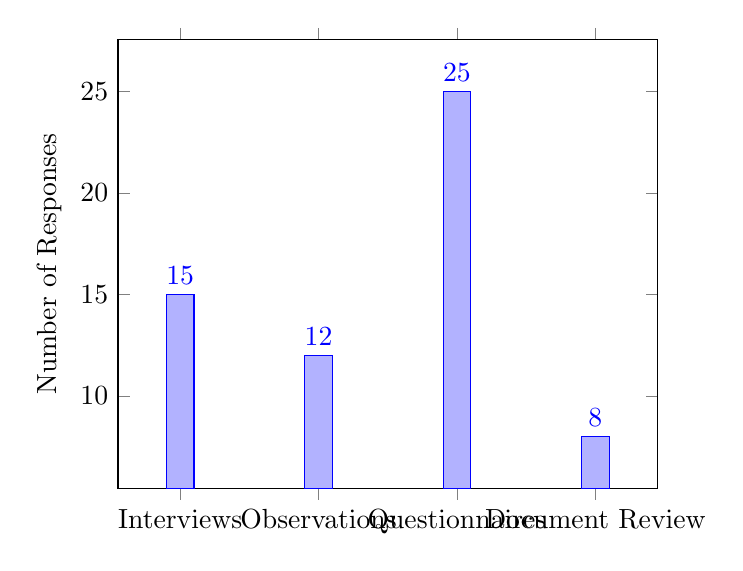
\begin{tikzpicture}
        \begin{axis}[
            ybar,
            enlargelimits=0.15,
            legend style={at={(0.5,-0.15)},
            anchor=north,legend columns=-1},
            ylabel={Number of Responses},
            symbolic x coords={Interviews,Observations,Questionnaires,Document Review},
            xtick=data,
            nodes near coords,
            nodes near coords align={vertical},
            ]
            \addplot coordinates {(Interviews,15) (Observations,12) (Questionnaires,25) (Document Review,8)};
        \end{axis}
    \end{tikzpicture}
    \caption{Bar Graph Showing Data Collection Responses for Weather-Pest Research}
\end{figure}

\begin{figure}[H]
    \centering
    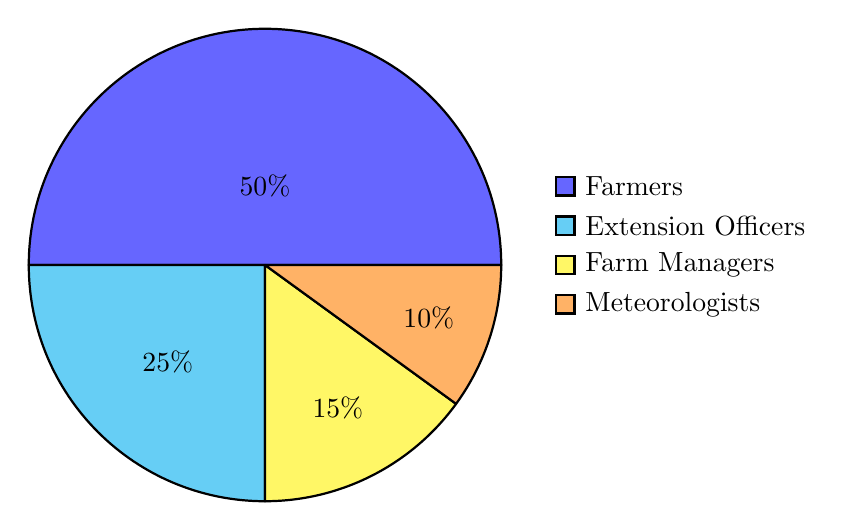
\begin{tikzpicture}
        \pie[text=legend]{
            50/Farmers,
            25/Extension Officers,
            15/Farm Managers,
            10/Meteorologists
        }
    \end{tikzpicture}
    \caption{Pie Chart Showing Specialized Participant Categories for Weather-Pest Research}
\end{figure}

\subsection{Phase 2: Quick Design}
After gathering weather-pest correlation requirements, a quick design is created focusing on:
\begin{itemize}
    \item Weather data integration architecture
    \item Pest/disease risk algorithm design
    \item Preventive alert generation logic
\end{itemize}

\subsection{Phase 3: Building the Prototype}
The initial prototype is constructed with specialized components:
\begin{itemize}
    \item Weather Data Module: API integration for localized forecasts
    \item Correlation Engine: Algorithms linking weather patterns to risks
    \item Alert Generation System: Logic for preventive alert creation
    \item Mobile Interface: Flutter-based application
    \item Backend: PHP API with MySQL database
    \item SMS Integration: Africa's Talking API for feature phone users
\end{itemize}

\subsection{Phase 4: Initial User Evaluation}
The prototype is evaluated specifically for:
\begin{itemize}
    \item Accuracy Testing: Comparing alerts with actual outbreaks
    \item Timing Evaluation: Assessing preventive lead time
    \item Usability Testing: Farmer comprehension of information
\end{itemize}

\subsection{Phase 5: Refining the Prototype}
Improvements are made based on evaluation feedback:
\begin{itemize}
    \item Adjusting correlation algorithm parameters
    \item Refining alert timing
    \item Simplifying information presentation
\end{itemize}

\subsection{Phase 6: Engineering the Final Product}
Upon validation, the final system is deployed with:
\begin{itemize}
    \item Optimized correlation algorithms
    \item Validated preventive alert timing
    \item User-tested interfaces
\end{itemize}

\section{System Architecture}
\begin{figure}[H]
    \centering
    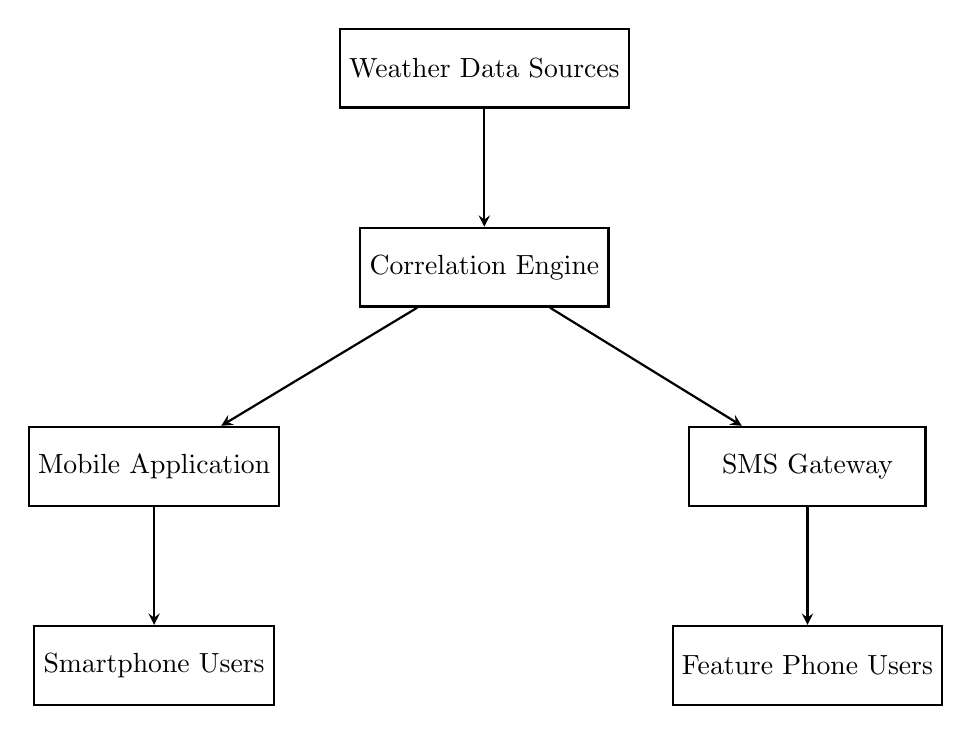
\begin{tikzpicture}[
        node distance=1.5cm and 1cm,
        box/.style={rectangle, draw=black, thick, minimum width=3cm, minimum height=1cm, text centered},
        arrow/.style={->, >=stealth, thick}
        ]

        % Nodes
        \node[box] (weather) {Weather Data Sources};
        \node[box, below=of weather] (correlation) {Correlation Engine};
        \node[box, below left=of correlation] (mobile) {Mobile Application};
        \node[box, below right=of correlation] (sms) {SMS Gateway};
        \node[box, below=of mobile] (user1) {Smartphone Users};
        \node[box, below=of sms] (user2) {Feature Phone Users};

        % Arrows
        \draw[arrow] (weather) -- (correlation);
        \draw[arrow] (correlation) -- (mobile);
        \draw[arrow] (correlation) -- (sms);
        \draw[arrow] (mobile) -- (user1);
        \draw[arrow] (sms) -- (user2);

    \end{tikzpicture}
    \caption{System Architecture for Weather-Pest Integrated Advisory Application}
\end{figure}

\section{Ethical Considerations}
Ethical guidelines are strictly followed with special considerations for:
\begin{itemize}
    \item Data Accuracy Responsibility: Preventing false alerts
    \item Informed Consent: Explaining experimental nature to participants
    \item Privacy: Securely handling location-specific data
\end{itemize}

\section{Anticipated Challenges}
\begin{itemize}
    \item Data Quality: Incomplete historical records
    \item Algorithm Accuracy: Developing accurate correlation models
    \item Farmer Trust: Building confidence in preventive alerts
    \item Microclimate Variability: Accounting for localized weather variations
\end{itemize}

\section{Conclusion}
The prototyping methodology is particularly suited for developing the specialized weather-pest integrated advisory application. The iterative approach allows continuous refinement of correlation algorithms based on field validation.

%%% Bibliography %%%%%%%%%%%%%%%%%%%%%%%%%%%%%%%%%%%%%%%%%%%%%%%%%%%%%%%%%%%%%%
\newpage
\phantomsection
\addcontentsline{toc}{chapter}{Bibliography}

\begin{thebibliography}{99}

\bibitem{MAAIF2019} Ministry of Agriculture, Animal Industry and Fisheries. \emph{Agricultural extension policy implementation framework}. MAAIF, Kampala, Uganda, 2019.

\bibitem{MAAIF2020} Ministry of Agriculture, Animal Industry and Fisheries. \emph{Agricultural Sector Strategic Plan 2020-2025}. Technical report, MAAIF, Kampala, Uganda, 2020.

\bibitem{UBOS2023} Uganda Bureau of Statistics. \emph{Statistical Abstract 2023}. UBOS, Kampala, Uganda, 2023.

\bibitem{ITU2023} International Telecommunication Union. \emph{ICT Statistics 2023}. ITU, Geneva, Switzerland, 2023.

\bibitem{FAO2020} Food and Agriculture Organization of the United Nations. \emph{Digital advisory services for smallholder farmers}. FAO, Rome, Italy, 2020.

\bibitem{FAO2022} Food and Agriculture Organization of the United Nations. \emph{State of Food and Agriculture 2022}. FAO, Rome, Italy, 2022.

\bibitem{WorldBank2021} World Bank. \emph{Enabling the business of agriculture report}. World Bank Group, Washington, DC, 2021.

\bibitem{WorldBank2022} World Bank. \emph{Digital agriculture in Africa: Opportunities and challenges}. World Bank, Washington, DC, 2022.

\bibitem{AgriculturalGrowth2022} Ministry of Agriculture, Animal Industry and Fisheries. \emph{Agricultural Growth Trends in Uganda}. Journal of Agricultural Economics, 10(2):1-15, 2022.

\bibitem{Lewis2019} Lewis, J. P. \emph{Project Planning, Scheduling, and Control}. 6th edition. McGraw-Hill Education, New York, USA, 2019.

\bibitem{FarmDrive2021} FarmDrive Ltd. \emph{Farmdrive: Data-driven credit scoring for smallholder farmers}. Available: \url{https://www.farmdrive.co.ke} (Accessed: 2025-11-04).

\bibitem{WeFarm2022} WeFarm Ltd. \emph{Wefarm: The world's largest farmer-to-farmer digital network}. Available: \url{https://www.wefarm.com} (Accessed: 2025-11-04).

\end{thebibliography}

%%% Index %%%%%%%%%%%%%%%%%%%%%%%%%%%%%%%%%%%%%%%%%%%%%%%%%%%%%%%%%%%%%%%%%%%%%
\newpage
\phantomsection
\addcontentsline{toc}{chapter}{Index}
\printindex

%%% Glossary %%%%%%%%%%%%%%%%%%%%%%%%%%%%%%%%%%%%%%%%%%%%%%%%%%%%%%%%%%%%%%%%%%
\newpage
\phantomsection
\addcontentsline{toc}{chapter}{Glossary}

\chapter*{Glossary}
\begin{description}
    \item[Smart Agriculture] The use of technology and data analysis to optimize agricultural processes.
    \item[Weather-Pest Integration] The correlation of meteorological data with pest and disease outbreak probabilities.
    \item[Preventive Farming] Agricultural practices focused on preventing problems before they occur.
    \item[Digital Extension Services] Technology-enabled agricultural advisory and support services.
    \item[Microclimate] The climate of a small, specific area that may differ from the surrounding region.
\end{description}

%%% Appendix %%%%%%%%%%%%%%%%%%%%%%%%%%%%%%%%%%%%%%%%%%%%%%%%%%%%%%%%%%%%%%%%%%
\appendix
\chapter{Questionnaire Template}
\section{Farmer Information Needs Assessment}
\begin{enumerate}
    \item What weather information do you currently use for farming decisions?
    \item How do you currently receive pest and disease advisories?
    \item Would you find weather-based pest alerts useful?
    \item What type of mobile device do you own?
    \item How would you prefer to receive agricultural advisories?
\end{enumerate}

\end{document}
